
\section{Creating a dataset of 4D scenes}
\label{sec:data}


\begin{figure}
    \centering
    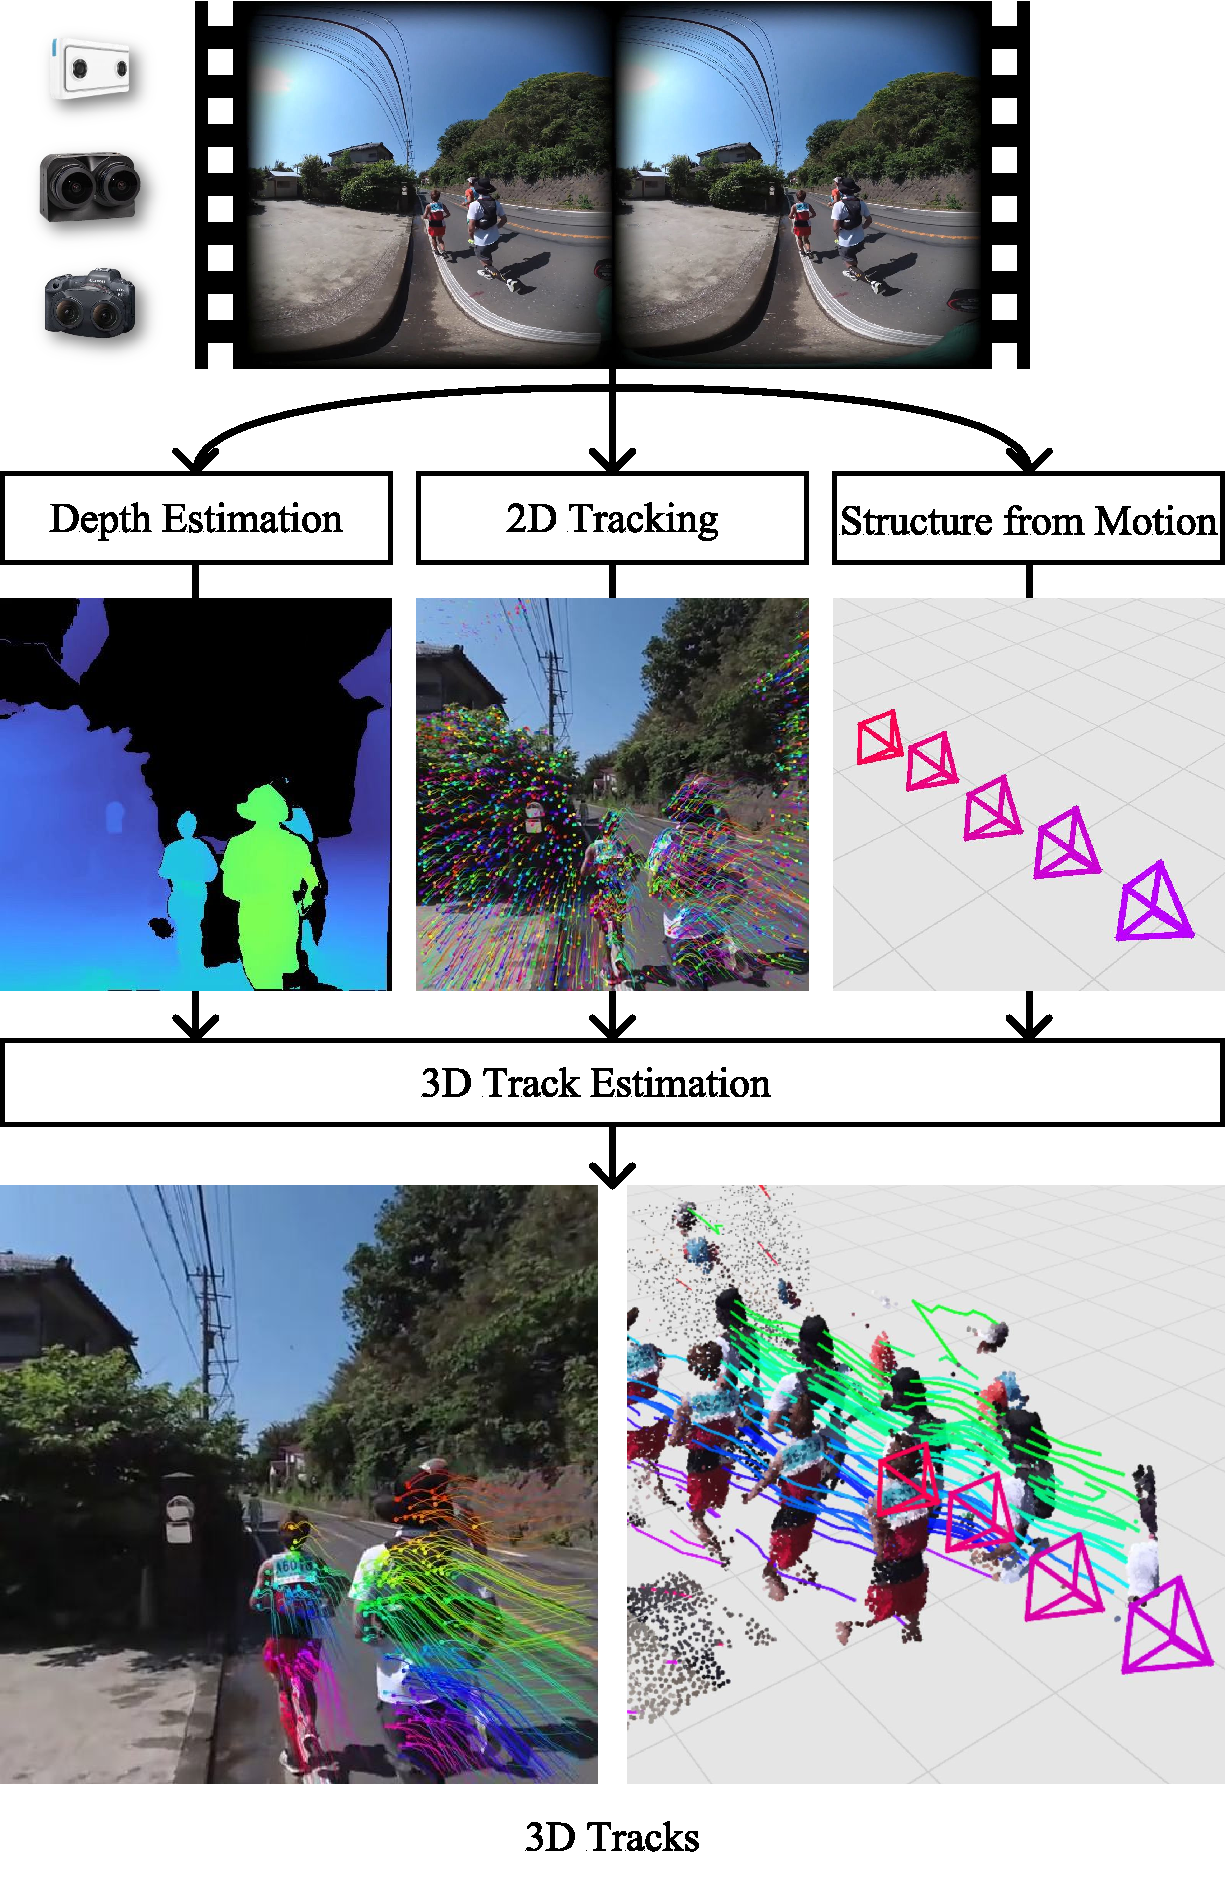
\includegraphics[width=\linewidth]{fig/data_processing_vertical.pdf}
    \vspace{-2em}
    \caption{\textbf{Data processing pipeline.} Our method starts with VR180 (wide-angle, stereoscopic) videos, and estimates metric stereo depth, 2D point tracks, and camera poses. These quantities allow the tracks to be lifted to 3D where they are filtered and denoised to produce world-space, metric 3D point trajectories.}
    \label{fig:data_pipeline}
\end{figure}

A core contribution of this work is a pipeline for extracting high-quality, pseudo-metric, 3D data from online stereoscopic fisheye videos (known as VR180 videos). 
High-resolution, wide field of view VR180 videos can be found readily online.
We show that this data is ideal for deriving rich dynamic 3D information that can power models for predicting geometry and motion from imagery.

Concretely, each instance of data starts as an $N$ frame stereo video consisting of left-right image pairs $\IB_i$ and $\IB'_i$ indexed by frame index $i\in[1,N]$. We convert these stereo pairs to a dynamic 3D point cloud with $K$ points in a world-space coordinate frame, where each point, indexed by $j\in[1,K]$, has a time-varying position $\pB_i^j$. 
As part of the process of generating this dynamic point cloud, we also extract a number of auxiliary quantities: (1) per-frame camera extrinsics, (the left camera's position $\cB_i$ and orientation $\RB_i$), (2) rig calibration for the stereo video giving the position $\cB_r$ and orientation $\RB_r$ of the right camera relative to the left camera, and (3) a per-frame disparity map $\DB_i$.


\subsection{Data Processing Pipeline} 

At a high level, our pipeline for converting a stereoscopic video into a dynamic point cloud involves estimating camera poses, stereo disparity, and 2D tracks, fusing these quantities into a consistent 3D coordinate frame, and performing several filtering operations to ensure temporal consistent, high-quality reconstructions (\Fig{data_pipeline}). In this section, we describe in detail the key components of this process. %


\medskip
\noindent \textbf{SfM.} 
We start by processing the sequence of stereo frames $\IB_i \leftrightarrow \IB_i'$ to produce camera pose estimates ($\cB_i, \RB_i$). We first use a SLAM method to divide the video into shots, as in~\cite{zhou2017scene}. For each shot, we run an incremental SfM algorithm similar to COLMAP~\cite{schonberger2016structure}. We initialize the stereo rig calibration $(\cB_r, \RB_r)$ to a rectified stereo pair with baseline $6.3$cm, but optimize for the calibration in bundle adjustment. In practice, we found that the exact stereo pair orientation can vary significantly from its nominal configuration and that optimizing the rig was critical for good results. 

\medskip 
\noindent \textbf{Depth Estimation.}
We next estimate a per-frame disparity map, operating on each frame independently. In particular, we use the estimated camera rig calibration $\cB_r, \RB_r$ to create rectified stereo pairs from the stereo fisheye video and estimate the per-frame disparity~$\DB_i$ with RAFT~\cite{sun2022disentangling,
sun2021autoflow,teed2020raft}. 

\medskip
\noindent \textbf{3D Track Estimation and Optimization.}  %
We extract long-range 2D point trajectories using BootsTAP~\cite{doersch2024bootstap}. Using the camera poses $\cB_i, \RB_i$ and disparity maps $\DB_i$, we unproject these tracked points into 3D space, turning each 2D track $j$ into a 3D motion trajectory $\pB^j_1, \ldots, \pB^j_N$
 across all frames. In general, each point will usually only be tracked in a subset of frames, but for simplicity, we describe the formulation as if all points are always visible. Moreover, since subsequent steps are done independently per-track, we drop the superscript $j$ in future references. 

Since stereo depth estimation is performed per-frame, the initial disparity estimates (and therefore, the 3D track positions) are likely to exhibit high-frequency temporal jitter. To compensate for potentially inconsistent disparity estimates, we formulate an optimization strategy that solves for a per-frame scalar offset $\delta_i \in \mathbb{R}$ that moves each point $\pB_i$ along the ray from camera location $\cB_i$ to $\pB_i$ at frame $i$. 
This ray is denoted $\rB_i = (\pB_i - \cB_i) / ||\pB_i - \cB_i||$, and we refer to the updated location as $\pB_i' = \pB_i + \delta_i \rB_i$. 

To ensure static points remain stationary while moving tracks maintain realistic, smooth motion, avoiding abrupt depth changes frame by frame, we design an optimization objective comprising three terms: a static loss $\mathcal{L}_{\mathsf{static}}$, a dynamic loss $\mathcal{L}_{\mathsf{dynamic}}$, and a regularization loss $\mathcal{L}_{\mathsf{reg}}$. The static loss $\mathcal{L}_{\mathsf{static}}$ minimizes jitter by encouraging points to remain close to each other in world space:
\begin{equation}
\mathcal{L}_{\mathsf{static}} = \sum_{i=1}^{N} \sum_{j=1}^{N} \frac{\| \mathbf{p}_i' - \mathbf{p}_j' \|^2}{N_p'^2}
\label{eq:objective_function}
\end{equation}
where $N_p' = \sum_{i=1}^N{\|\mathbf{p}'_i\|} / N$ is a normalizing factor.
The dynamic loss term reduces jitter by minimizing acceleration along the camera ray through a discrete Laplacian operator:
\begin{equation}
\mathcal{L}_{\mathsf{dynamic}} = \sum_{i=1}^{N} \sum_{\Delta\in\mathcal{W}} \left[ \left( \mathbf{p}_{i+\Delta}' - 2\mathbf{p}_i' + \mathbf{p}_{i-\Delta}' \right)^\top \mathbf{r}_i \right]^2
\label{eq:dynamic_objective}
\end{equation}
where the acceleration along the ray is calculated over
multiple window sizes $\mathcal{W}=\{1,3,5\}$.


The two loss terms are weighted by a track-dependent function, $\sigma(m)$, where $m$ is a measure of the motion magnitude of the track. Motion is measured in 2D rather than 3D because distant points can appear to have a larger 3D motion due to noise amplification at low disparities.
Specifically, we project the 3D motion trajectory between time $i - w_o$ and the current time $i$ into 2D image-space at time $i$, %
and calculate the track's motion magnitude $m$ as the 90$^{th}$ percentile of the track's trail length across all frames. The track trail length for a frame is measured by projected 3D points along the track to the current frame as if the camera is \emph{static} in a window of $w_o=16$ frames, 
\begin{equation}
\label{eqn:trail_length_def}
    m = \mathsf{Percentile}_{i=1:N}^{90}\left[\max_{w=1:w_o}\|\pi_i(\pB_i) - \pi_i(\pB_{i-w})\|\right]
\end{equation}
where $\pi_i(\cdot)\in \mathbb{R}^2$ gives the projected pixel location of a 3D point on camera $\cB_i$'s image plane.
The weighting function $\sigma(m)$ is defined as $\sigma(m) = \frac{1}{1 + \exp(m - m_0)}$ where $m_0 = 20$. 
Finally, to encourage faithfulness to the originally estimated disparities, we regularize the displacements in disparity space:
\begin{equation}
    \mathcal{L}_{\mathsf{reg}} = \lambda_{\mathsf{reg}} \sum_{i=1}^{T} \left( \frac{1}{\delta_i + \|\mathbf{p}_i-\mathbf{c}_i\|} - \frac{1}{\|\mathbf{p}_i-\mathbf{c}_i\|} \right)^2,
\end{equation}
where use of disparity space reflects the fact that the measurements themselves originate as disparities. Practically, the impact of the use of disparity is that larger deviations are tolerated at more distant points, where depth is intrinsically more uncertain.

The full objective function is
\begin{equation}
\min_{\{\delta_i\}_{i=1}^N} \sigma(m)\mathcal{L}_{\mathsf{static}} + (1-\sigma(m))\mathcal{L}_{\mathsf{dynamic}} + \mathcal{L}_{\mathsf{reg}}.
\label{eqn:objective}
\end{equation}
We set $\lambda_{\mathsf{reg}}=10^{-4}$ and optimize Eqn.~\ref{eqn:objective} using Adam with a learning rate of 0.05 for 100 steps.
The effect of track optimization is shown in \Fig{track_optimization}. The optimized motion is smoother and does not contain high frequency noise.


\begin{figure}[t]
    \centering
    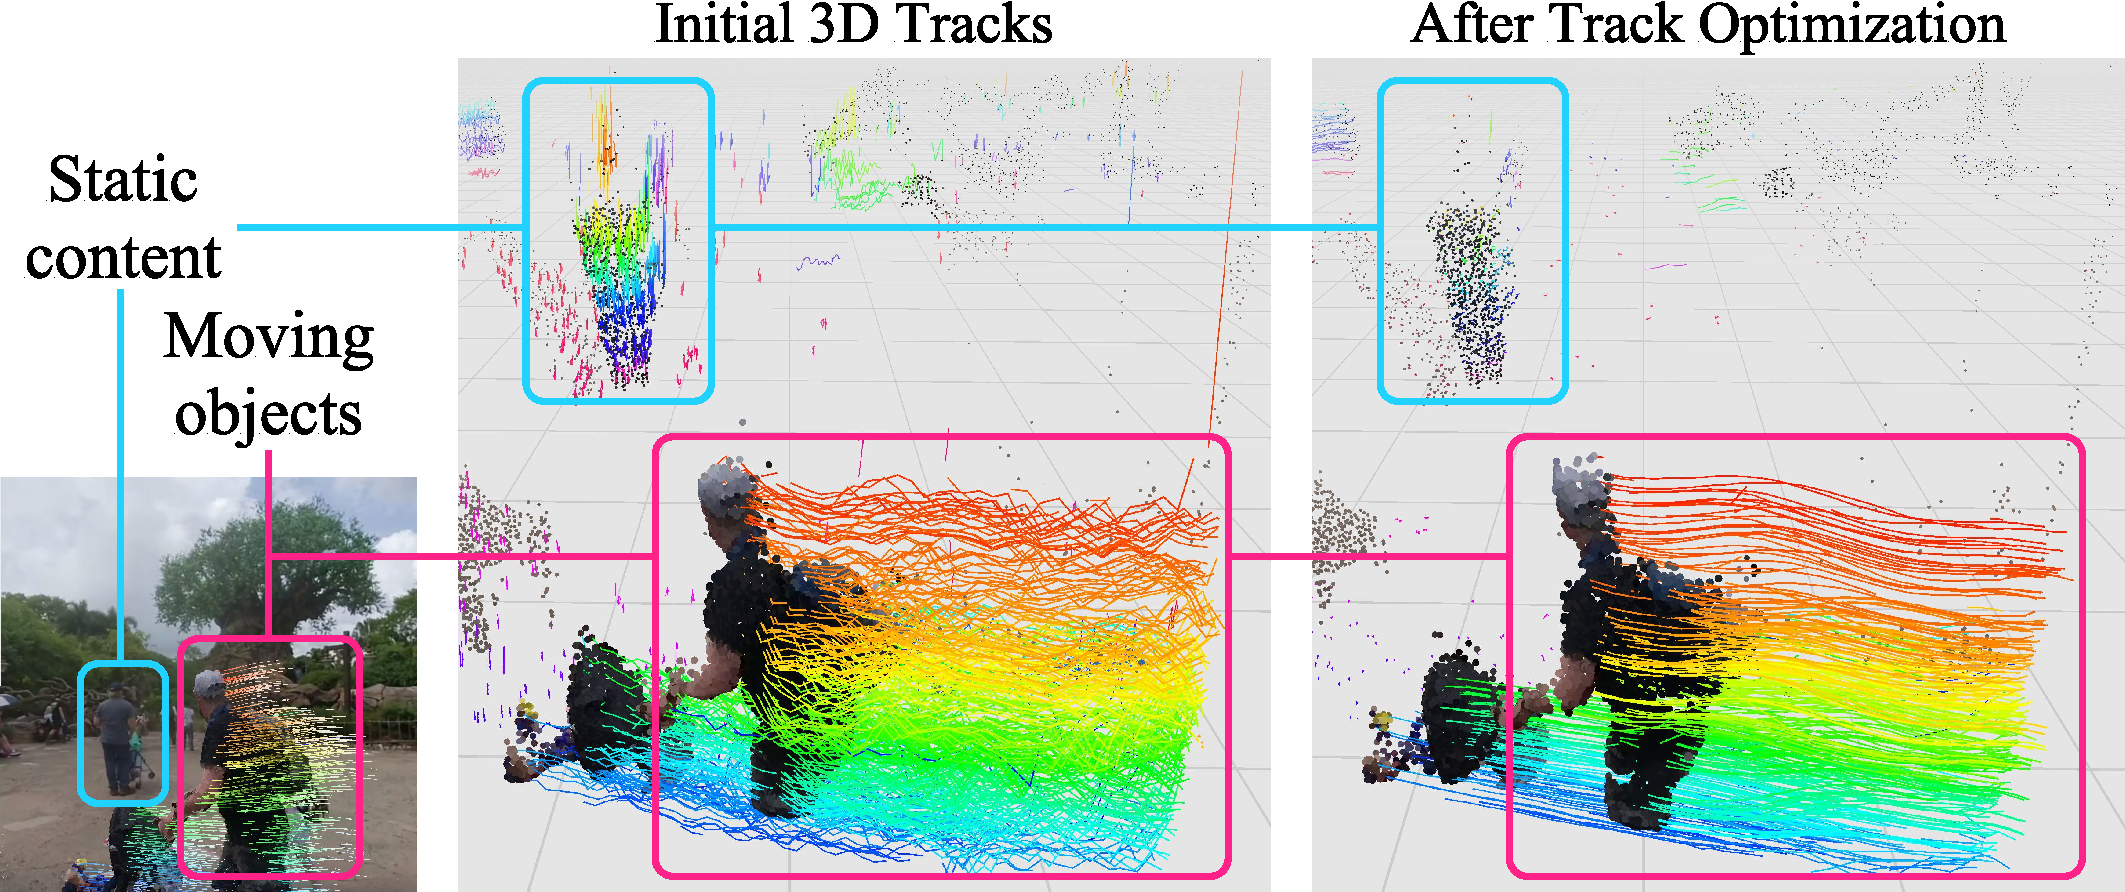
\includegraphics[width=\linewidth]{fig/optimization.pdf}
    \caption{\textbf{Effect of track optimization.} Comparing motion trajectories before and after track optimization, we see that optimization resolves the high frequency jitter along camera rays, affecting both static and dynamic content. After optimization, static content has static tracks, and dynamic tracks are less noisy.}
    \label{fig:track_optimization}
\end{figure}


\begin{figure*}[t]
\vspace{-1em}
    \centering
    \includegraphics[width=\textwidth]{fig/diversity-highres.pdf}
    \caption{\textbf{Diverse motion:} \dataset captures a wide variety of types of moving objects, from swimming fish, to walking pedestrians, moving vehicles, and a farmer sowing seeds. It includes source videos captured with both stationary (left) and moving (right) cameras.}
    \label{fig:motion_distribution}
\end{figure*}
\medskip
\noindent \textbf{Implementation details.} %
{\it Shot-selection.} Rather than work with the full video, we break the footage into discrete, trackable shots using ORB-SLAM2's stereo estimation mode~\cite{murartal2015orbslam} following~\cite{zhou2018stereo}. 
{\it Field of View.} While estimating pose, we use a $140^\circ$ FoV fisheye format, which we found to capture more of the (usually static) background and less of the (often dynamic) foreground, yielding more reliable camera poses. 
{\it Stereo Confidence Checks.} We discard pixels where the $y$-component of RAFT flow is more than 1 pixel (since rectified stereo pairs should have perfectly horizontal motion) and where the stereo cycle consistency error is more than 1 pixel (since such pixels are unreliable). 
{\it Dense 2D tracks.} To get dense tracks, we run BootsTAP with dense query points: for every 10th frame, we uniformly initialize $128\times128$ query points on frames of resolution 512 $\times$ 512. We then prune redundant tracks that overlap on the same pixel.
{\it Drifting tracks.} Since 2D tracks can drift on textureless regions, we discard moving 3D tracks that correspond to certain semantic categories (\textit{e.g.}, ``walls'', ``building'', ``road'', ``earth'', ``sidewalk''), detected by DeepLabv3~\cite{chen2017rethinking} on ADE20K classes~\cite{zhou2017scene, zhou2019semantic}.

\medskip
\noindent \textbf{Filtering details.} A fraction of the video clips that are processed may be unsuitable because they either (1) are not videos, and are entirely static images, (2) contain cross-fades, or (3) have text or other synthetic graphics. To discard text and title sequences, we avoid creating video clips from the start and ends of the source videos. We identify cross-fades by running SIFT~\cite{lowe2004sift} matching through the video at multiple temporal scales and discarding video clips with static camera but with fewer than 5 SIFT matches between frames that are 5 seconds apart.



\begin{figure}[t]
    \centering
    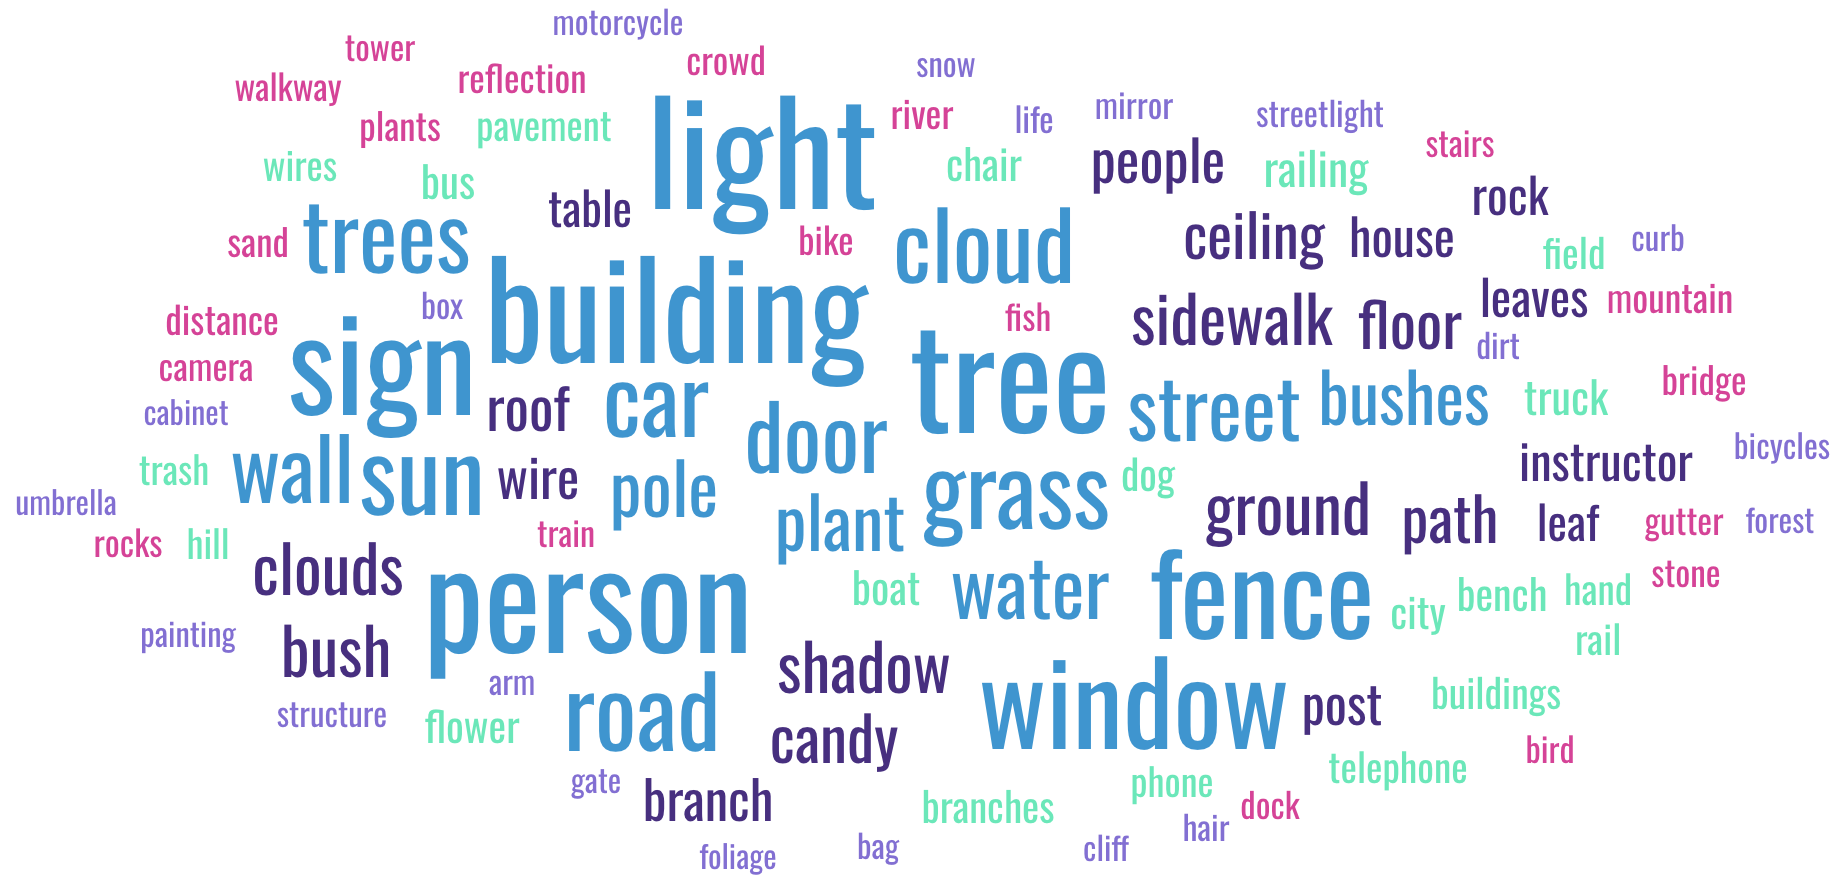
\includegraphics[width=\linewidth]{fig/wordcloud.png}
    \caption{\textbf{Diverse scene content:} A word cloud of captioned frames from our dataset shows our data is diverse, including a variety of common objects seen in videos.}
    \label{fig:wordcloud}
\end{figure}


\subsection{Stereo4D Dataset}

\Fig{motion_distribution} illustrates a subset of videos and reconstructions from a dataset processed with the above pipeline, encompassing more than 100K clips capturing everyday scenes and activities. To visualize the range of content, we used an automatic captioning system to generate captions for the dataset and created a word cloud (\Fig{wordcloud}) highlighting the most frequently observed objects.





